\chapter{Results and Discussion}

\section{Model Validation}
\label{sec:section14}
Both the baseline model, derived from the MASER-in-a-Shoebox
dimensions\autocite{ng2023maser}, and the initialised model used for genetic
optimisation successfully supported resonant modes at approximately 1.45 GHz,
operating in the characteristic $\text{TE}_{01\delta}$ mode.

\begin{figure}[htbp]
  \centering
  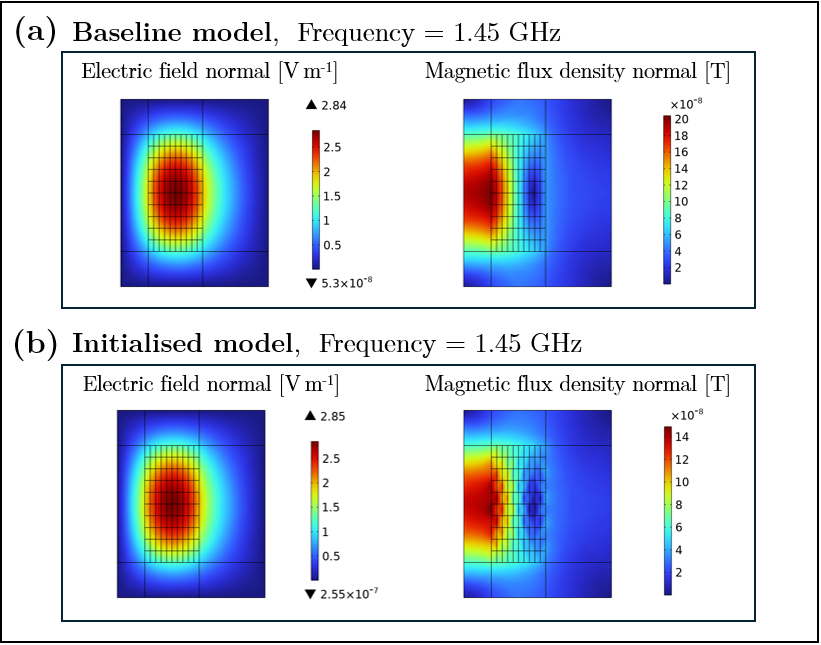
\includegraphics[width=0.8\textwidth]{figures/figure11.png}
  \caption{
    Comparison of the electric field normal and magnetic flux density normal for
    (a) the baseline model and (b) the initialised model, both resonating at
    1.45 GHz. The baseline configuration replicates dimensions from the
    MASER-in-a-Shoebox study\autocite{ng2023maser}, while the initialised model
    uses a checkerboard dielectric pattern. Both exhibit strong field
    confinement within the dielectric region and excitation of the
    $\text{TE}_{01\delta}$ mode.
  }
  \label{fig:figure11}
\end{figure}

To validate correct mode excitation and field behaviour, the electromagnetic
field distributions of both the baseline and initialised models were examined in
COMSOL. In both cases, the $\text{TE}_{01\delta}$ mode was successfully
identified at a resonant frequency near 1.45 GHz. This mode is characterised by
strong azimuthal symmetry in the magnetic field and minimal radial electric
field components, consistent with theoretical expectations.

Figures \ref{fig:figure11}(a) and (b) display the magnetic field intensity
distributions for the baseline and initialised models, respectively. In both,
the magnetic field is strongly confined within the dielectric resonator region,
while the electric field remains weak at the cavity boundaries, confirming that
the desired mode has been correctly isolated. These field patterns provided
confidence that the subsequent Purcell factor and quality factor calculations
are based on physically valid solutions.

A quantitative comparison between the MASER-in-a-Shoebox-derived baseline model
and the initialised model used for the genetic algorithm is presented in Table
\ref{table3}. Both models were designed to resonate at 1.45 GHz and employed
identical simulation domains, meshing parameters, and boundary conditions.
Importantly, these models were computed without including the dielectric loss
tangent of the STO. This omission was deliberate, as it allowed for an isolated
evaluation of electromagnetic confinement and field distribution without
introducing material-dependent damping. However, this also means the reported
quality factors represent unloaded or idealised values, not reflective of the
actual physical losses in STO.

The mode volume was calculated using the magnetic field distribution and the
standard definition described in the Methods section. Subsequently, the
$\frac{Q}{V_m}$ was computed for each model. As shown in Table \ref{table3}, the
baseline model exhibited a higher Purcell factor than the initialised model,
indicating slightly improved field confinement and reduced mode volume.

\section{Genetic Algorithm Results}
\label{sec:section15}
Following the establishment of a validated initialised model, the genetic
algorithm was executed to optimise the geometry of the dielectric resonator with
the objective of maximising the Purcell factor. Over the course of 250
generations, with a population size of 20, the GA iteratively modified the
permittivity profile of the resonator using a binary-coded 10×10 subgrid. This
allowed the algorithm to explore a wide design space while maintaining the
resonant frequency near the target 1.45 GHz. Figure \ref{fig:figure12} presents
the evolution of the maximum and average $\frac{Q}{V_m}$ over all generations.
The rapid increase in both metrics within the first 50 generations indicates
efficient convergence toward favourable geometries. Subsequent generations
continued to produce incremental gains, with the best-performing geometry
emerging around generation 200. This optimised configuration resulted in a
substantial increase in Purcell factor compared to both the baseline and the
initialised models. Over the whole GA, $\frac{Q}{V_m}$ appears to increase by
600\%, which is a very surprising result.

\begin{figure}[htbp]
  \centering
  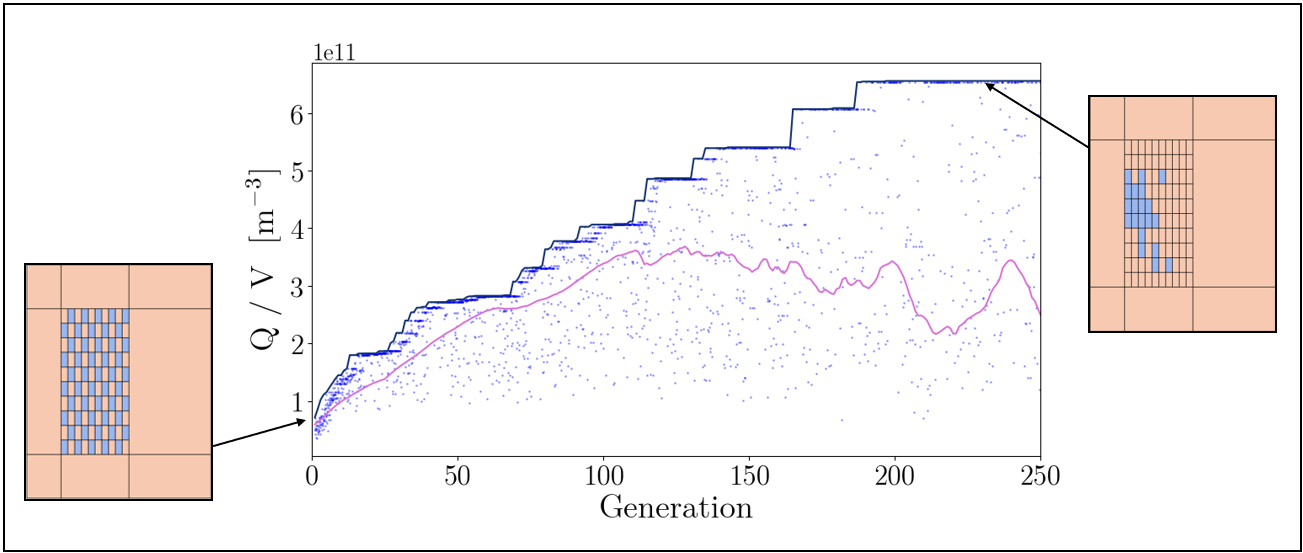
\includegraphics[width=1\textwidth]{figures/figure12.png}
  \caption{
    Evolution of the genetic algorithm over 250 generations. The highest
    $\frac{Q}{V_m}$ found in each generation is shown by the dark blue line,
    while the pink line shows the moving average $\frac{Q}{V_m}$. All individual
    simulation results are plotted as small blue dots. The initial and final
    dielectric configurations, corresponding to the start and end of the
    optimisation, are shown alongside the plot.
  }
  \label{fig:figure12}
\end{figure}

To better understand how the GA achieved this enhancement, the individual
components of the Purcell factor were also tracked. Figure \ref{fig:figure13}(a)
shows the $Q_f$ over all iterations (i.e. every individual evaluated across all
generations). The spread of values reflects the diversity of explored
geometries. Similarly, Figure \ref{fig:figure13}(b) displays the $V_m$ over
time. A gradual decrease in $V_m$ can be observed across the optimisation
process, reflecting a supposed improved electromagnetic confinement within the
dielectric structure.

\begin{figure}[htbp]
  \centering
  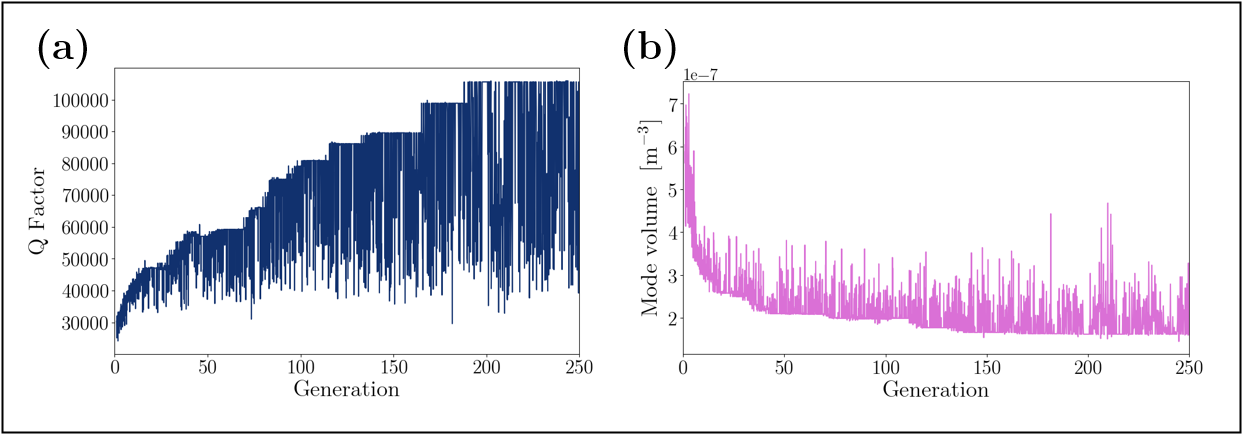
\includegraphics[width=1\textwidth]{figures/figure13.png}
  \caption{
    (a) Quality factor and (b) mode volume as functions of generation number
    during the genetic algorithm run. As the optimisation progresses, the
    quality factor generally increases while the mode volume decreases,
    contributing to the overall improvement in the Purcell factor.
  }
  \label{fig:figure13}
\end{figure}

In Figure \ref{fig:figure14}(a), the resonant frequency of all evaluated
geometries is shown. Most newly generated configurations initially resonated at
frequencies significantly offset from the 1.45 GHz target. However, the
iterative permittivity-scaling loop, incorporating Lagrange interpolation,
effectively returned these frequencies to the desired range within a small
number of iterations. The convergence of resonant frequencies across the
optimisation process demonstrates that the interpolation method was successfully
able to correct deviations and ensure consistent evaluation of the Purcell
factor across varying geometries. Figure \ref{fig:figure14}(b) shows the
evolution of $\alpha$ (and therefore $\varepsilon$) over the course of the GA.
$\alpha$ quickly increased to over 1.6 in over 50 generations, corresponding to
a global increase in the resonators dimensions. Each simulation started with
$\alpha=1$ before the scaling occurs which is why the graph continually returns
to $\alpha=1$.

\begin{figure}[htbp]
  \centering
  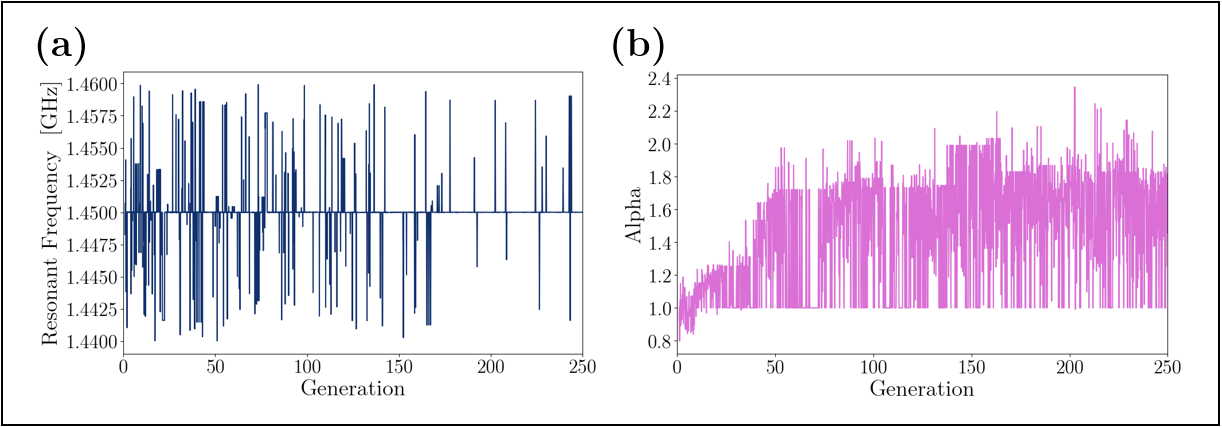
\includegraphics[width=1\textwidth]{figures/figure14.png}
  \caption{
    (a) Resonant frequency and (b) permittivity scaling factor $\alpha$ as
    functions of generation number during the genetic algorithm run. The
    frequency plot shows consistent convergence toward the target value of 1.45
    GHz, while the increase in $\alpha$ reflects a progressive rise in the
    scaled relative permittivity values of both air and dielectric regions.
  }
  \label{fig:figure14}
\end{figure}

The final optimised configuration, extracted at generation 208, exhibited the
highest Purcell factor achieved during the GA run. Its corresponding field
distribution, visualised in COMSOL, confirmed strong magnetic field confinement
within the dielectric region, consistent with a well-coupled resonant mode. This
configuration was then used as the input for the \texttt{QuantumCumulants.jl}
simulation, enabling the evaluation of practical masing performance.

\begin{figure}[htbp]
  \centering
  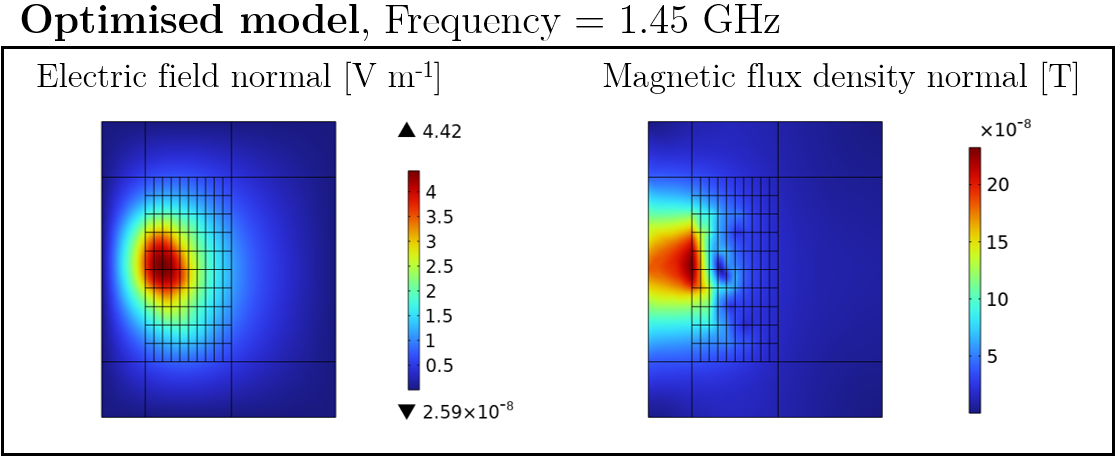
\includegraphics[width=0.8\textwidth]{figures/figure15.png}
  \caption{
    Electric field normal and magnetic flux density normal distributions of the
    optimised model at 1.45 GHz. The optimised configuration supports the
    $\text{TE}_{01\delta}$ mode, with strong magnetic field confinement within
    the dielectric structure.
  }
  \label{fig:figure15}
\end{figure}

\section{Quantum Cumulants Results}
\label{sec:section16}
To assess how geometric optimisation of the dielectric resonator influences
practical masing performance, both the baseline and optimised configurations
were simulated using the \texttt{QuantumCumulants.jl} package. Each model’s
calculated quality factor $Q_f$ and mode volume $V_m$ were used to derive the
photon decay rate (Equation \ref{eq:kappa}) and the light–matter coupling
strength (Equation \ref{eq:g53}), which were then implemented as input
parameters in the Julia simulation. These values directly influence the
intracavity dynamics and ultimately the masing output power.

\begin{figure}[htbp]
  \centering
  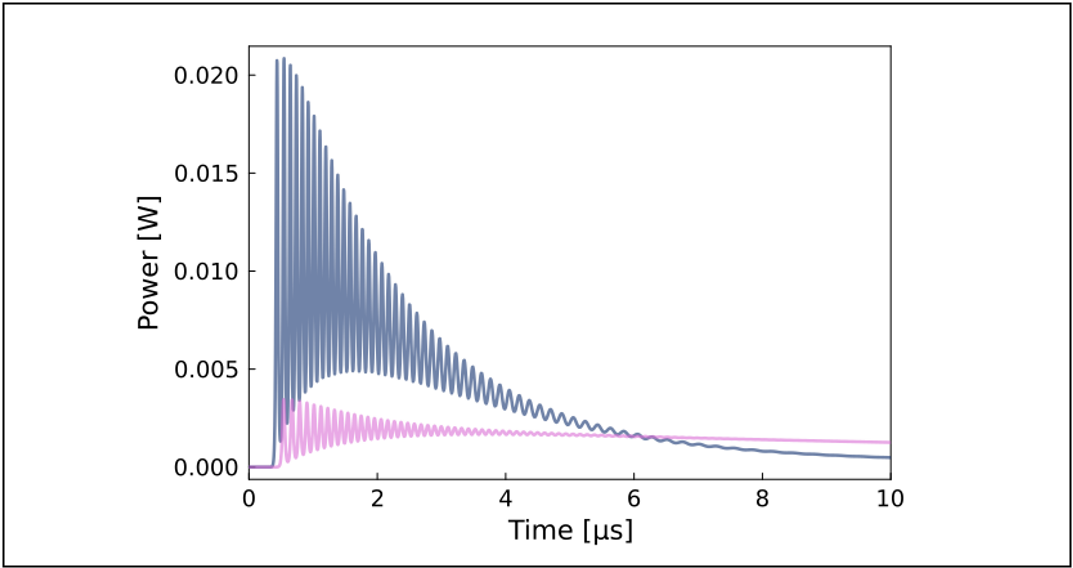
\includegraphics[width=0.8\textwidth]{figures/figure16.png}
  \caption{
    Simulated output power over time for the optimised configuration (dark blue)
    and initial configuration (pink). While the optimised resonator shows higher
    peak power and faster masing onset, these results are purely comparative and
    do not represent actual output power values. The model serves as a relative
    performance indicator under idealised conditions.
  }
  \label{fig:figure16}
\end{figure}

The simulations tracked the time evolution of the intracavity photon number
$\langle a^\dagger a \rangle$, from which the masing output power was calculated
via Equation \ref{Pout}.

As shown in Figure \ref{fig:figure16}, the optimised configuration produced a
noticeably higher peak output power and reached its maximum value more rapidly
than the baseline model. This trend is attributed to the enhanced Purcell factor
of the optimised geometry, which increases the rate of spontaneous emission into
the cavity mode and promotes faster buildup of coherent photons. It is important
to note, however, that the output power profiles generated using
QuantumCumulants.jl are not intended to represent absolute real-world
measurements. Instead, they provide a useful visual and comparative framework
for evaluating relative differences in masing performance between
configurations. Throughout the simulated free-evolution period, the optimised
model consistently outperformed the baseline in terms of sustained output power,
indicating more efficient and robust masing behaviour under the idealised
conditions used in the model.

These results demonstrate that geometric optimisation, even using a simple
pixelated subgrid and binary material assignment, can lead to meaningful
performance improvements at the device level. The table below, Table
\ref{table3}, summarises the key quantitative metrics extracted from the
baseline and optimised models. All values reflect the unloaded (lossless)
simulations as the dielectric loss tangent was excluded from both COMSOL and
Julia simulations to isolate geometric contributions.

\begin{figure}[htbp]
  \centering
  \captionof{table}{A comparison of the three losses models.}
  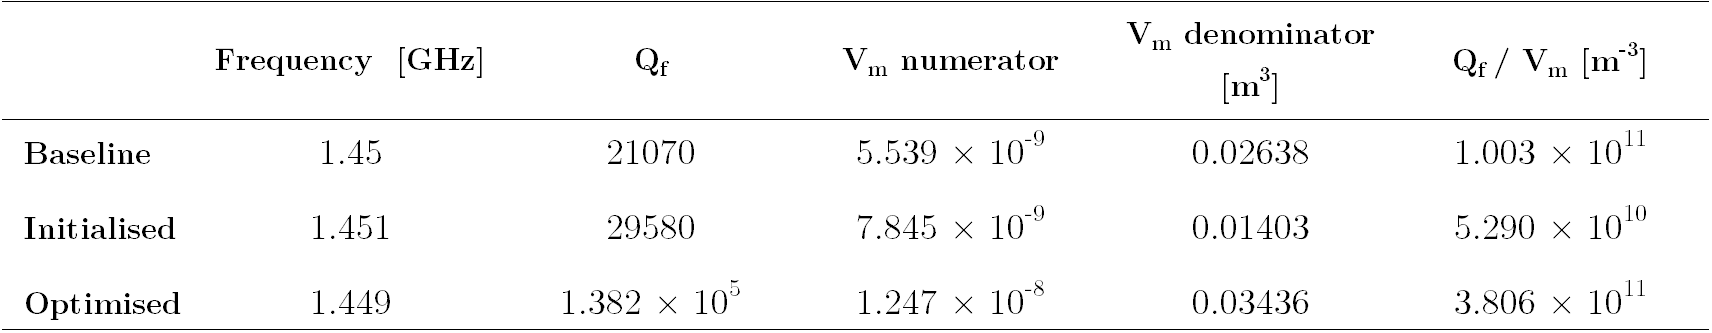
\includegraphics[width=0.9\textwidth]{tables/table3.png}
  \label{table3}
\end{figure}

\section{Limitations of Results}
\label{sec:section17}
While the results presented demonstrate clear improvements in resonator
performance through geometric optimisation, several important limitations must
be acknowledged, most notably, the simplified treatment of material losses. In
all COMSOL simulations used throughout this project, the dielectric loss tangent
of STO was deliberately omitted to try and retain simplicity and increase the
speed at which the GA runs. Ultimately, this resulted in idealised and
unrealistic performances. In practical implementations, STO exhibits a
non-negligible loss tangent (on the order of $10^{-4}$ to $10^{-3}$), which
would substantially reduce the real-world $Q_f$, especially at GHz frequencies.
The equation for the total Q factor considering all major methods of loss can be
seen in Equation \ref{eq:Qtot}.

\begin{equation}
  \frac{1}{Q_{\text{tot}}} =
    \frac{1}{Q_{\text{ohm}}}
    + \frac{1}{Q_{\text{diel}}}
    + \frac{1}{Q_{\text{rad}}}
  \label{eq:Qtot}
\end{equation}

Where $Q_{\text{ohm}}$ is the $Q_f$ of the cavity walls, $Q_{\text{diel}}$ is
the $Q_f$ of the dielectric (determined by the loss tangent, $\tan\delta$), and
$Q_{\text{rad}}$ is the $Q_f$ of radiative losses. This method assumes
$1/Q_{\text{tot}} = 1/Q_{\text{ohm}}$.

This omission affects the physical accuracy of both the COMSOL and Julia
simulations. In COMSOL, losses are only accounted for via the impedance boundary
condition applied to the copper cavity walls, which introduces conductive losses
through surface current dissipation. Additionally, any radiative losses due to
imperfect field confinement are inherently captured by the finite simulation
domain and open boundary conditions. However, dielectric losses, often the
dominant loss channel in high-permittivity materials like STO, are not
represented, and therefore the reported Purcell factors are overestimated
relative to real-world performance.

In fact, when the optimised configuration was simulated with a dielectric which
included a loss tangent. The gains in Purcell factor were found in lossy
conditions and the Purcell factor was lower than that of the baseline model.
Therefore, this model would not outperform the baseline model in experimental
conditions.

\section{Loss-included Models}
\label{sec:section18}
To move toward a more physically realistic optimisation, an updated version of
the genetic algorithm (GA) was developed with the aim of including the loss
tangent of the dielectric material. This was implemented by assigning a complex
relative permittivity (in the $tan\delta$ column of Appendix \ref{table4}) to
the dielectric regions within the COMSOL model, introducing an imaginary
component proportional to the specified loss tangent.

In principle, this would allow the GA to optimise not just for electromagnetic
confinement but also for geometries that minimised overall dissipative loss.
However, this modification introduced a significant computational challenge: in
the presence of realistic dielectric loss, the solver consistently found
incorrect modes. Many configurations either failed to converge to a valid mode
or converged to unintended resonant solutions with poor confinement and
irrelevant field distributions. This instability made the fitness function
unreliable, preventing the GA from effectively progressing. As a result, the
optimisation loop was unable to identify meaningful high-performing geometries
under lossy conditions. This is all highly likely caused by an unidentified bug
in my code.

\begin{figure}[htbp]
  \centering
  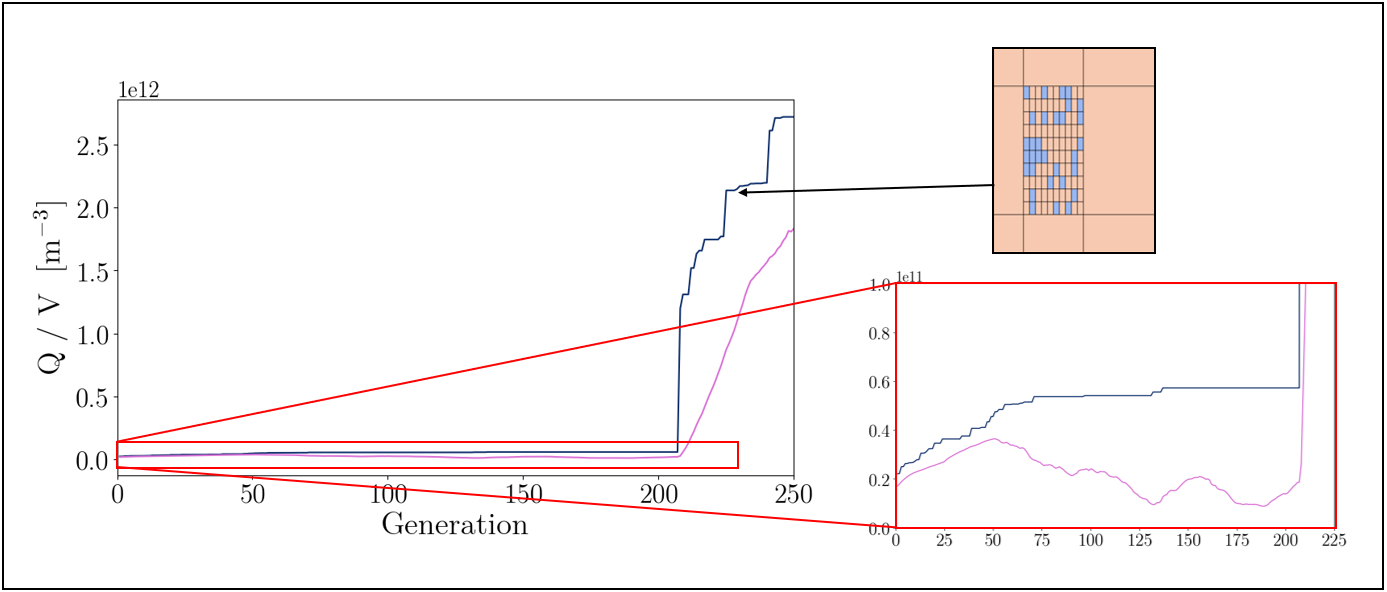
\includegraphics[width=1\textwidth]{figures/figure18.png}
  \caption{
    Progression of the genetic algorithm under lossy conditions. The dark blue
    line shows the highest $\frac{Q}{V}$ recorded at each generation, while the
    pink line represents the average $\frac{Q}{V}$ across all simulations. The
    inset zooms in on the slow initial progress of the algorithm, followed by a
    sudden breakthrough in performance after approximately 200 generations. The
    final configuration is also shown.
  }
  \label{fig:figure18}
\end{figure}

The configurations returned from the failed model were extracted to try to
identify where the root of the issue was. In Figure \ref{fig:figure18}, even
though the $F_P$ does increase significantly towards the end of the GA, this is
due to mode switching. This is confirmed by Figure \ref{fig:figure17}, which
shows the resonator is not longer operating in the $\text{TE}_{01\delta}$ mode.
Mode switching during the GA is a problem as the model loses its consistency, so
any results are invalid.

\begin{figure}[htbp]
  \centering
  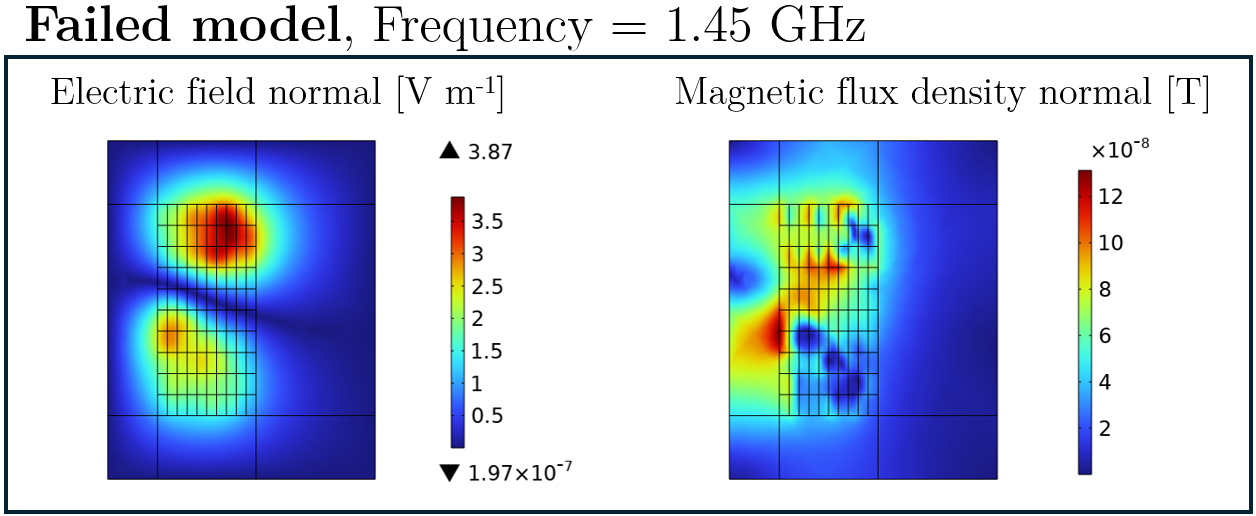
\includegraphics[width=0.8\textwidth]{figures/figure17.png}
  \caption{
    Electric field normal and magnetic flux density normal for a failed
    configuration that resonated at 1.45 GHz. Its shape can be seen in
    \ref{fig:figure18}. The magnetic flux density shows poor confinement within
    the dielectric region, with significant energy leakage into surrounding
    areas. This indicates weak field–material interaction, resulting in a low
    Purcell factor and ineffective masing behaviour.
  }
  \label{fig:figure17}
\end{figure}

To verify that these failures were not due to the unfeasibility of enhancing the
Purcell factor in lossy configurations, manual simulations were performed in
order to find more optimal geometries. Several configurations were found to
exhibit Purcell factors higher than that of the baseline MASER-in-a-Shoebox
model. One result is displayed in Figure \ref{fig:figure20}.

\begin{figure}[htbp]
  \centering
  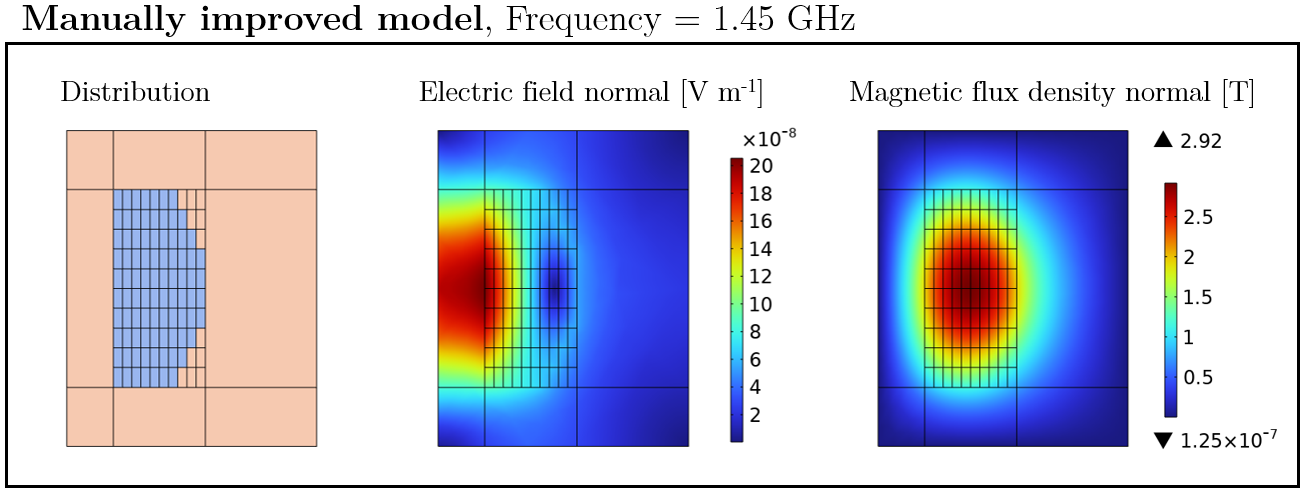
\includegraphics[width=0.8\textwidth]{figures/figure20.png}
  \caption{
    Manually optimised configuration demonstrating improved field confinement.
    The distribution shows the dielectric domains (blue).
  }
  \label{fig:figure20}
\end{figure}

These results confirmed that performance improvements were physically achievable
even with realistic losses. A comparison to the baseline model is shown in Table
\ref{table5}.

\begin{figure}[htbp]
  \centering
  \captionof{table}{
    Comparison of baseline and manually optimised configurations in the presence
    of dielectric loss.
  }
  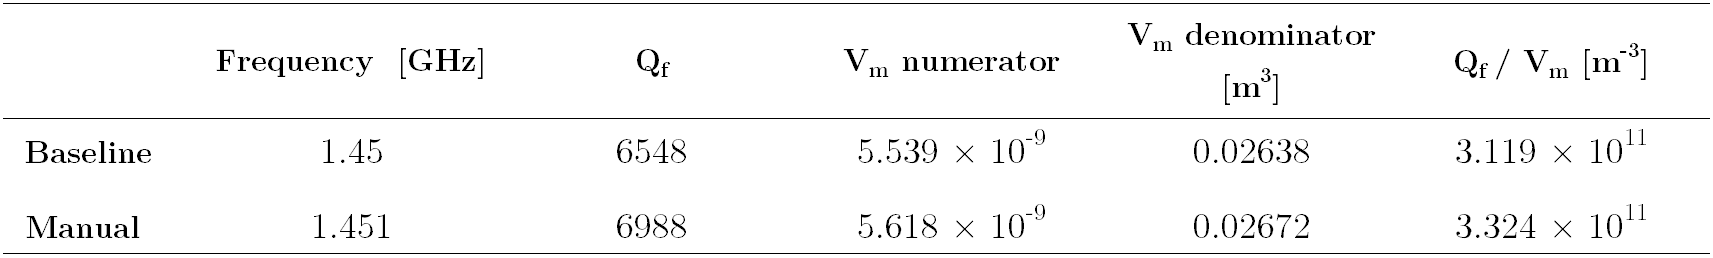
\includegraphics[width=1\textwidth]{tables/table5.png}
  \label{table5}
\end{figure}

Due to time constraints of the project, a full redesign of the frequency
correction procedure could not be implemented. However, a feasible solution was
proposed: frequency tuning with Q-neutral permittivity adjustment.

This method still involves adjusting the global permittivity to bring the
resonant frequency to 1.45 GHz, but critically it does so without altering the
total quality factor $Q_{\text{total}}$ of the dielectric material. This would
require incorporating the filling factor, $\eta$, which quantifies the fraction
of the electromagnetic field energy stored within the dielectric:

\begin{equation}
  \eta = \frac{\int_{\text{dielectric}} \varepsilon |\mathbf{E}|^2 \, dV}
              {\int_{\text{total}} \varepsilon |\mathbf{E}|^2 \, dV}
\end{equation}

Given this, the total quality factor Q of the system can be expressed as:

\begin{equation}
  \frac{1}{Q_{\text{tot}}} =
    \frac{\eta}{Q_\text{diel}} + \frac{1}{Q_{\text{other}}}
    = \eta~tan\delta_{diel}+ \frac{1}{Q_{\text{other}}}
\end{equation}

Where $Q_{\text{other}}$ represents other losses such as conduction ($Q_{ohm}$)
and radiation ($Q_{rad}$).

$Q_{\text{tot}}$ needs to remain fixed and while the frequency is scaled to the
target frequency.

By decoupling frequency correction from loss scaling, the proposed method allows
more stable exploration of the design space, preserving the integrity of the
fitness function and enabling meaningful optimisation even under lossy
conditions. Implementing this strategy would require integrating filling factor
calculations into the GA loop and defining the dielectric loss independently of
the real permittivity scaling. While more complex, it offers a promising path
forward for loss-aware resonator optimisation.

\section{Additional Further Work}
\label{sec:section19}
Several other opportunities for further development remain. One such improvement
is the implementation of a ‘surface energy’ factor within the genetic
algorithm’s fitness evaluation. The current framework allows for isolated
dielectric domains with disconnected regions that may not form a coherent 2D
structure. While such configurations can yield high Purcell factors, they will
be physically difficult to manufacture. Introducing a ‘glueing’ penalty or
reward term could encourage the evolution of continuous, manufacturable
geometries by favouring designs that form a single contiguous resonator body.
Whether such isolated domains could be made physically viable remains an open
question. One speculative approach might involve embedding discrete dielectric
regions within a surrounding resin that has electromagnetic properties closely
matching those of air. This would theoretically preserve the field distribution
observed in simulation, but such materials would require extremely low loss
tangents and negligible permittivity. In practice, enforcing coherent shapes
through algorithmic constraints or penalty terms is likely a much more feasible
path forward.

Another avenue for future work is expanding the optimisation into full 3D
modelling. While this study relied on COMSOL’s 2D axisymmetric mode, due to its
efficiency and alignment with cylindrical geometries, more complex or asymmetric
dielectric shapes may yield even greater improvements in Purcell factor.
Accessing these designs requires abandoning rotational symmetry and operating
within a full 3D simulation framework. The increased computational load
associated with 3D simulation would necessitate a more efficient integration
pipeline than was available in this project.

This may be implementable using the COMSOL LiveLink\texttrademark{} for
MATLAB\textregistered{} that represents an improvement over the Java API used in
this study. MATLAB\textregistered{}’s powerful numerical libraries, intuitive
syntax, and data handling capabilities are far better suited to genetic
algorithms and other optimisation routines. MATLAB\textregistered{}’s
environment would allow easier integration of adaptive mutation strategies,
multi-objective fitness functions, and visualisation of convergence trends.
Unfortunately, the MATLAB\textregistered{} LiveLink\texttrademark{} package
requires an additional paid licence, which was not purchased for this project
due to its high price and initial unawareness of its benefits. As a result, the
project proceeded using the COMSOL Java API, which, while functional, proved
more cumbersome and less flexible for advanced algorithmic control.

Looking further ahead, machine learning (ML) techniques could offer an extension
to this optimisation framework. A trained surrogate model, for instance, could
rapidly estimate Purcell factors for proposed geometries without requiring a
full COMSOL simulation at each step. This could accelerate convergence and
enable exploration of even larger and more complex design spaces. Combining
machine learning with LiveLink\texttrademark{} for MATLAB\textregistered{} would
allow for powerful hybrid approaches, such as reinforcement learning-based
geometry generation or Bayesian optimisation over a learned performance surface.

\section{Scientific and Practical Implications}
\label{sec:section20}
From a scientific perspective, this outcome reinforces a common challenge in
cavity QED and microwave engineering: the trade-off between field confinement
and loss minimisation. High confinement geometries often exacerbate losses
unless materials are carefully chosen or cooling is applied. This is consistent
with trends in the literature, where many high-Q devices rely on cryogenic
operation, ultra-low-loss dielectrics like sapphire, or careful modal
engineering (e.g., whispering gallery or anapole modes) to suppress
dissipation\autocite{fedotov2007anapole}. In terms of data quality,
uncertainties stem not from numerical error, since COMSOL’s eigenfrequency
solver is highly accurate. But rather from physical assumptions such as perfect
material behaviour, and the neglect of thermal effects.

This project has highlighted the potential of automated shape optimisation for
electromagnetic structures using genetic algorithms, offering a computational
route to discovering non-intuitive geometries. From an innovation and industry
perspective, this method, if made loss-aware, could support the development of
miniaturised, room-temperature MASERs with practical applications in quantum
sensing, deep-space communication, and ultra-low-noise amplifiers. However,
reaching this point will require further integration of material science (for
low-loss dielectrics) and experimental feedback (to validate optimised
geometries).

In summary, while the project successfully demonstrates an increase in Purcell
factor under idealised conditions, the realistic impact of loss limits the
viability of the discovered designs without further refinement. These findings
are therefore preliminary but insightful, pointing the way to more physically
accurate optimisation strategies in the next generation of MASER design.
